\documentclass[a3paper]{article}
\usepackage[margin=.25in]{geometry}
\usepackage[sets,operators,adversary,advantage,probability]{cryptocode}
\usepackage{tikz}
\usepackage{amsmath}
\usepackage{amsthm}
\usepackage{hyperref}
\newcommand{\pcas}{~\highlightkeyword{as}}
\newtheorem{theorem}{Theorem}
\newtheorem{claim}{Claim}
\theoremstyle{definition}
\newtheorem{definition}{Definition}
\newcommand\lit[1]{\ensuremath{\mathtt{#1}}}
\renewcommand\O[1]{\ensuremath{\mathsf{#1}}}
\newcommand{\M}[1]{\ensuremath{\text{\texttt{#1}}}}
\newcommand{\n}[1]{\ensuremath{\mathit{#1}}}
\tikzstyle{package} = [inner sep=1pt,align=center,rounded corners,draw,minimum width=2cm,minimum height=1cm,font=\small]
\tikzstyle{onarrow} = [inner sep=1pt,font=\scriptsize,anchor=west,at start,align=left,fill=white]
\title{G_Sim_FreeXORIdeal Game}
\begin{document}
\maketitle
\begin{center}
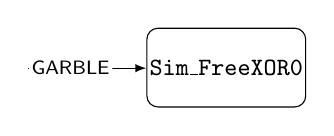
\begin{tikzpicture}
\node[anchor=south west,align=center,package,minimum height=1cm,fill=white] (node0) at (3.5,0.5) {\M{Sim\_FreeXOR0}};\draw[-latex,rounded corners] (2,1) -- node[onarrow] {\O{GARBLE}} (3.5,1);
\end{tikzpicture}

\end{center}
\begin{pchstack}
\input{Package_Sim_FreeXOR0_in_G_Sim_FreeXORIdeal_lossy.tex}
\pchspace
\end{pchstack}
\end{document}
